\section*{Chapter~2~~Technical~background}
\setcounter{section}{2} \setcounter{subsection}{0} 
\setcounter{table}{0} \setcounter{figure}{0} \setcounter{equation}{0} \setcounter{definition}{0}
\addcontentsline{toc}{section}{\textbf{Chapter~2~~Technical~background}}

\subsection{Topic material}

\subsubsection{Basics of Bluetooth Low Energy}
\noindent Bluetooth Low Energy (BLE) is often the technology of choice for networks where energy-efficient and cost-effective communication is paramount. This is especially common with low-cost, energy-constrained devices like temperature sensors that capture specific data attributes and wirelessly transmit this information to user devices, like smartphones. BLE operates using three dedicated radio frequency (RF) channels (37, 38, and 39) for advertising, which is the process of broadcasting the presence of a BLE device to initiate a connection \cite{gomez2012overview}. These are known as the advertising channels. Once a connection is established, the remaining channels, known as data channels, are used for the ongoing communication between devices.

\vspace{4pt}

The typical communication protocol in a BLE network encompasses four main stages: advertising, connecting, pairing, and data accessing \cite{wu2020blueshield}. The advertising stage is where the BLE device announces its availability to connect. In the connecting phase, a user device responds to this advertisement, establishing a bidirectional link. Pairing is the next crucial step, where security credentials are exchanged, forming the foundation for a secure communication. Finally, in the data accessing stage, the authenticated user device is able to read or write the data from or to the BLE device. \textbf{Figure 2-1} shows a typical network packet during the BLE communication, which includes data with time-series features such as packet number, timestamp, and payload data.

\begin{figure}[H]
    \centering
    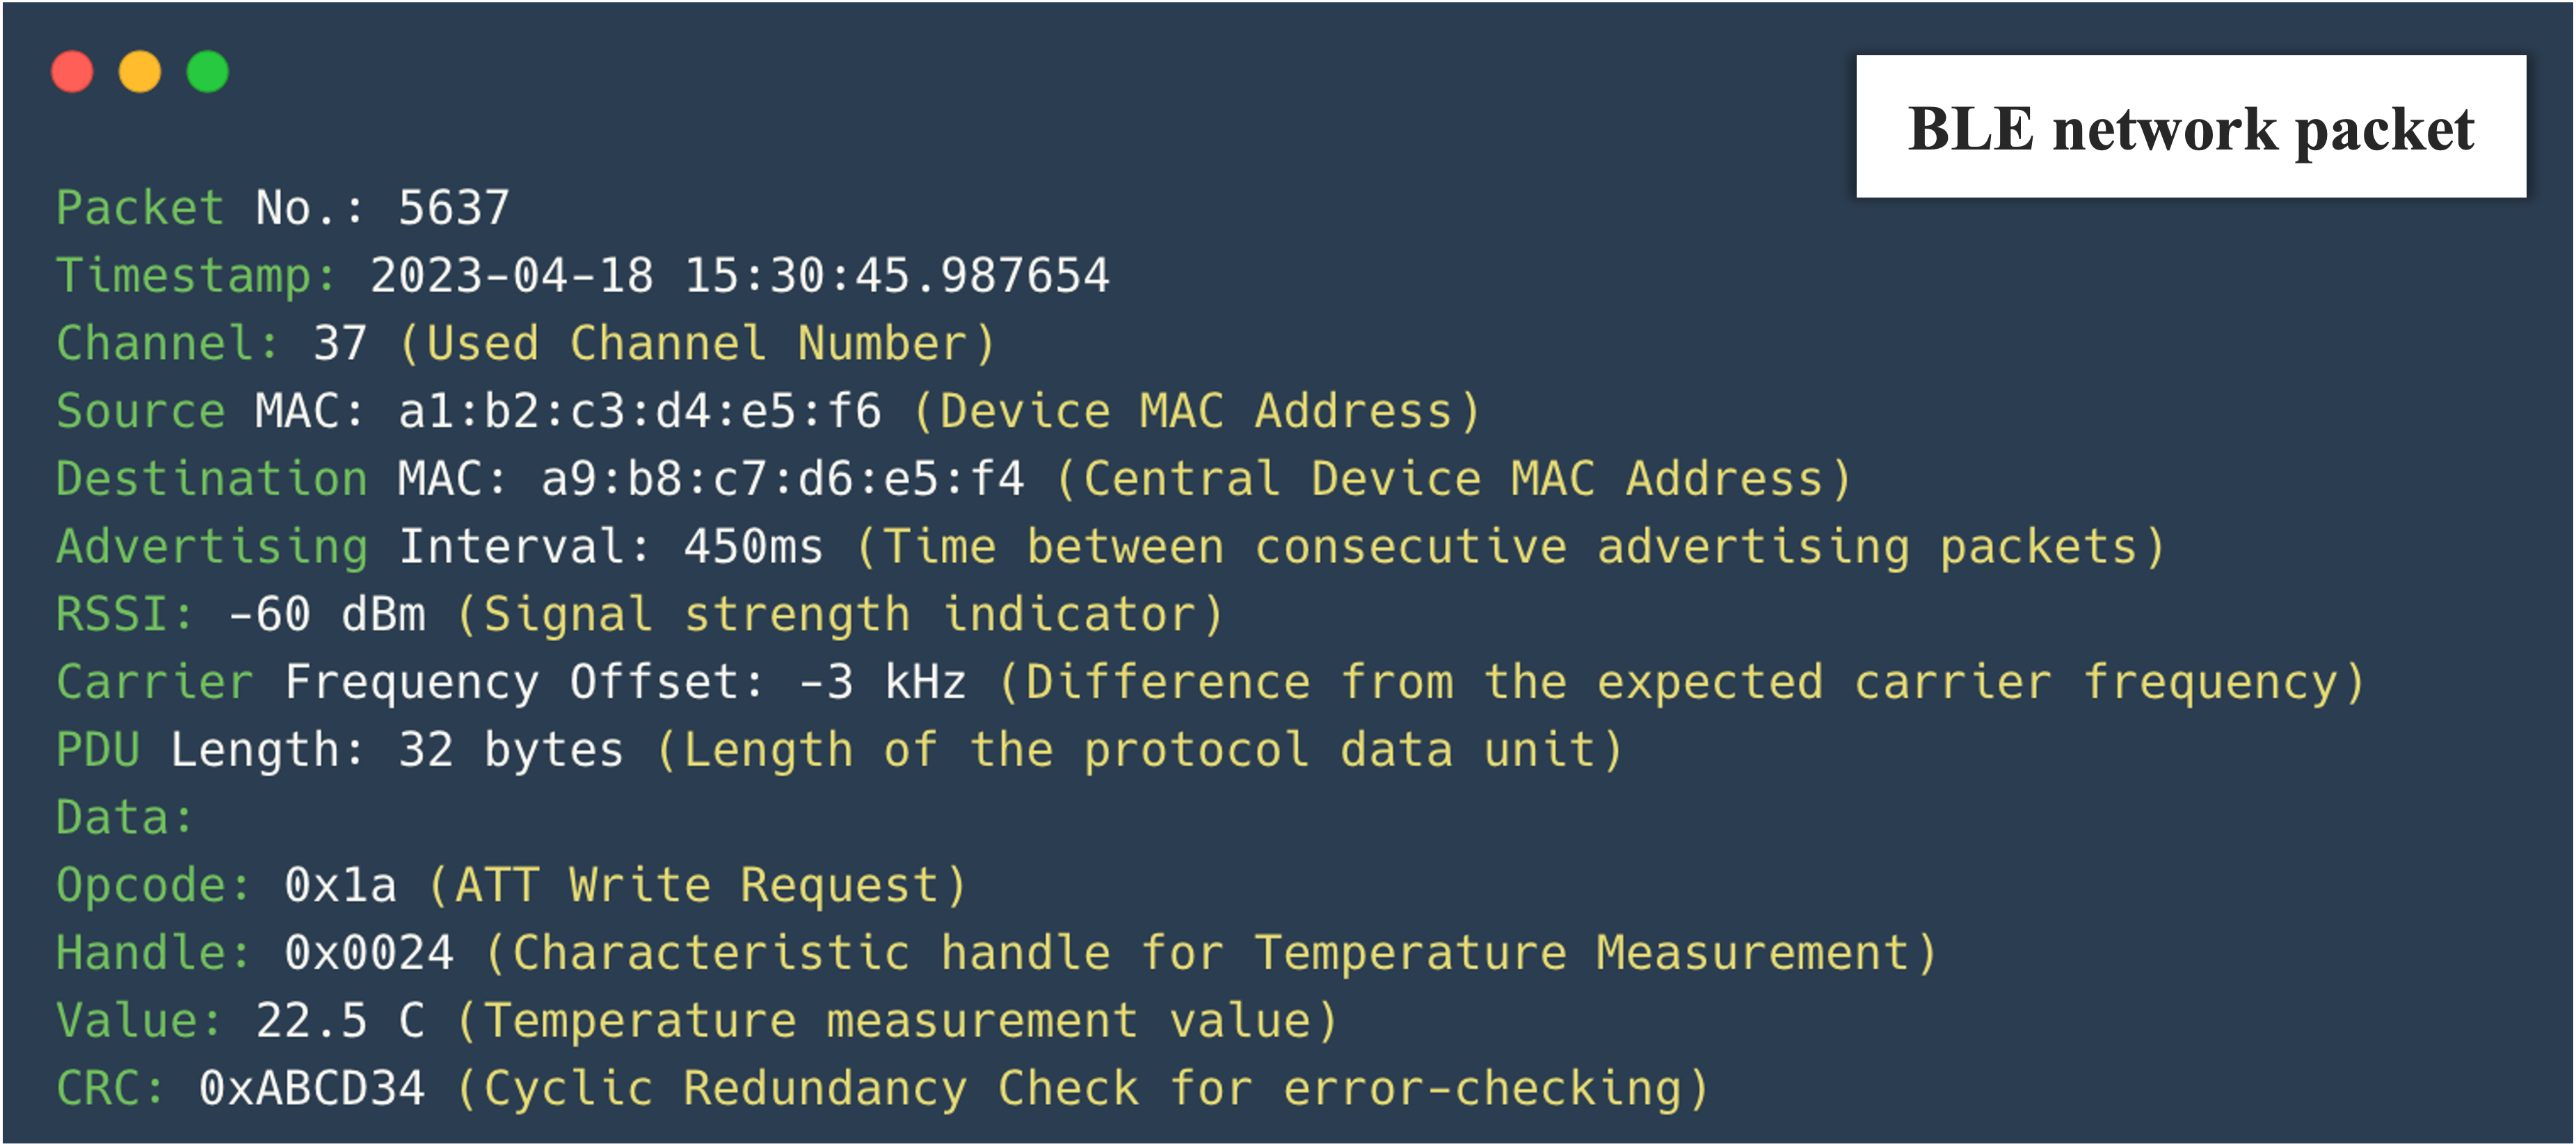
\includegraphics[width=1\linewidth]{FZU thesis templete//Fig/fig2-1.png}
    \caption{Sample data of a typical BLE network package.}
    \label{fig-2-1}
\end{figure}


\subsubsection{Spoofing Attacks in BLE Networks}

\noindent The spoofing attack is a type of cybersecurity attack wherein an attacker impersonates a legitimate BLE device or network entity \cite{zhang2017secure}. In such attacks, the perpetrator typically masquerades as a trusted BLE device using forged information, such as a spoofed MAC address or other identifying details, as illustrated in \textbf{Figure 2-2(a)}. In the context of a spoofing attack, the cyber-physical features of the BLE network are notably impacted, leading to significant deviations from typical benign scenarios. For instance, an anomalous shift in the RSSI (Received Signal Strength Indicator) values of the advertising packets can signal the presence of a spoofing attack, as depicted in \textbf{Figure 2-2(b)}. These deviations provide critical indicators that can be used to effectively identify potential malicious activity \cite{cai2024securing}.

\begin{figure}[H]
    \centering
    \resizebox{\textwidth}{!}{
    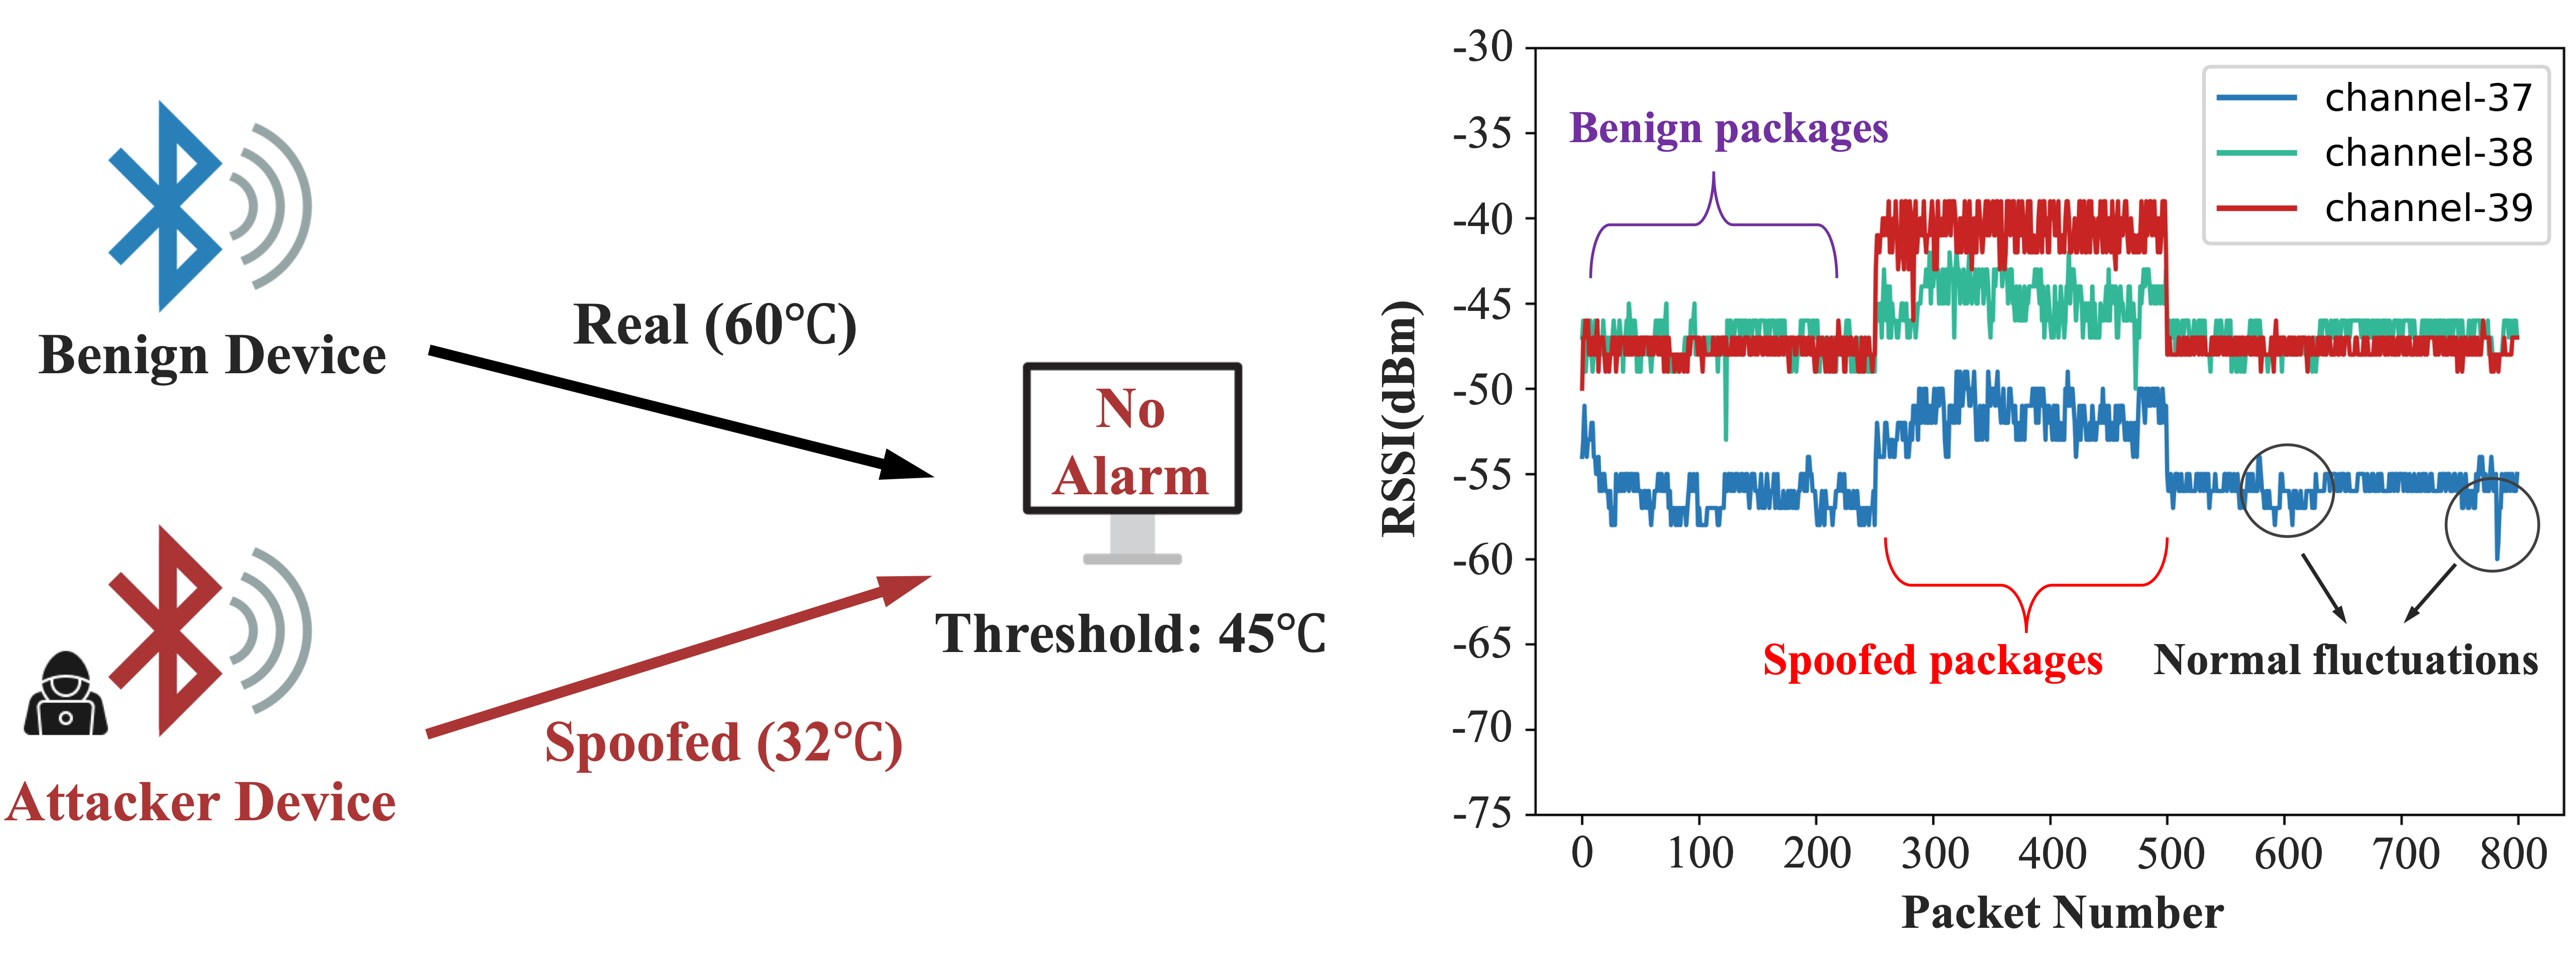
\includegraphics[width=1\linewidth]{FZU thesis templete//Fig/fig2-2.png}
    }
    \caption{(a) Spoofing attack in BLE sensor network and (b) observed RSSI values during attack simulation.}
    \label{fig-2-1}
\end{figure}

\noindent Given the unique characteristics of BLE networks, this project has successfully identified and utilized four key cyber-physical features to enhance the detection algorithm and to facilitate the training of learning models:

\begin{itemize}[leftmargin=0.1cm]
    \setlength{\itemsep}{-0.1cm}
    \item \textbf{Used Channel Numbers (UCN):} These denote the specific data channels employed during the transmission of BLE packets, crucial for analyzing communication patterns.
    \item \textbf{Advertising Interval (INT):} This measures the temporal interval between consecutive packets transmitted on the same advertising channel, vital for detecting timing anomalies.
    \item \textbf{Received Signal Strength Indicator (RSSI):} This feature represents the signal-to-noise ratio gleaned from packet exchanges, providing insights into the physical layer connectivity.
    \item \textbf{Carrier Frequency Offset (CFO):} Refers to the discrepancy between the expected and the actual carrier frequencies used in BLE communications, indicating potential frequency drifts or unauthorized channel usage.
\end{itemize}


\subsubsection{Related Research Findings}

\noindent The BLE specifications \cite{specification} provide a range of authentication mechanisms theoretically designed to prevent spoofing attacks. However, these mechanisms often fail to achieve their intended purpose in practice due to three main reasons: 

\begin{itemize}[leftmargin=0.1cm]
    \setlength{\itemsep}{-0.1cm}
    \item \textbf{(1) Limited Device I/O Capabilities: }A significant number of BLE devices have limited I/O capabilities, which precludes them from utilizing any robust authentication mechanisms. It is not surprising that recent research has shown that over 80\% of current BLE devices communicate with user devices in plaintext without any form of authentication \cite{bsecurity}.
    \item \textbf{(2) Persistent Security Vulnerabilities:} For BLE devices that do implement various security measures, there are still numerous attack vectors at both the protocol level and application level that malicious actors can exploit to conduct spoofing attacks \cite{wu2020blueshield}.
    \item \textbf{(3) Insufficient User Awareness:} Users of BLE devices may lack awareness or the technical knowledge required to enable and configure security features properly, leading to increased susceptibility to spoofing attacks \cite{casar2022survey}.
\end{itemize}

\vspace{-4pt}

\noindent Additionally, the challenge of implementing software-based solutions (i.e., firmware updates for BLE devices or software patches on user devices) to these security vulnerabilities is compounded by four major practical challenges:

\vspace{-4pt}

\begin{itemize}[leftmargin=0.1cm]
    \setlength{\itemsep}{-0.1cm}
    \item \textbf{(1) Ineffectiveness Against Zero-Day Exploits:} The nature of software patches does not allow them to preemptively protect against zero-day vulnerabilities, which can be immediately exploited by attackers upon discovery \cite{stellios2019advanced}.
    \item \textbf{(2) Fragmented Update Ecosystem:} The diversity in BLE device manufacturers leads to a fragmented ecosystem for firmware updates, which complicates the process of applying uniform security patches across devices.
    \item \textbf{(3) Legacy Device Constraints: }A considerable number of legacy BLE devices in use are incapable of being updated due to outdated I/O capabilities, leaving them vulnerable to new exploits.
    \item \textbf{(4) Resource Constraints for Update Dissemination:} Many manufacturers of BLE devices may face resource constraints that impede the timely development and distribution of necessary firmware updates, further exacerbating security challenges \cite{antonioli2020key}.
\end{itemize}

\subsection{Technical material}

% \noindent Throughout the development of the BLE network testbed and the subsequent collection of the network dataset, this project employed a variety of technical tools, such as attacker platforms and network sniffers, to facilitate data acquisition and analysis. Given the wide range of tools and methods utilized, a comprehensive explanation of each is beyond the scope of the main text. Detailed descriptions and justifications for these tools are therefore provided in \textbf{Appendices 1}.


\noindent Throughout the development of the BLE network testbed and the subsequent collection of the network dataset, this project employed a variety of technical tools to facilitate data acquisition and analysis. Given the extensive range of tools and methodologies utilized, a comprehensive explanation of each is beyond the scope of the main text. Detailed descriptions and justifications for these tools are therefore provided in \textbf{Appendices 1}. Below are examples of the categories of technical tools used:

\vspace{-4pt}

\begin{itemize}[leftmargin=0.1cm]
    \setlength{\itemsep}{-0.1cm}
    \item \textbf{Attacker Platforms:} Tools such as Mirage \cite{sun2020towards}, Ostinato \cite{khamaiseh2019detecting}, and custom scripts designed to emulate spoofing attack scenarios.
    \item \textbf{Network Sniffers:} Tools like Wireshark, Ubertooth, BLE-Analyzer-PRO and HCI snoop log.
    \item \textbf{Data Acquisition Systems:} Automated systems like nRF Connect for data logging and analysis.
    \item \textbf{Simulation Software:} Network simulators like GNS3 \cite{neumann2015book} used for virtual testing and modeling.
\end{itemize}


% \vspace{6pt}

% A detailed discussion on the specific applications and operational details of the technical tools utilized within our research framework will be discussed in \textbf{Section 4.1}. This section delves into the integration of each tool into our experimental setup, emphasizing their significant contributions to the robustness and precision of our data collection efforts. Furthermore, it elaborates on how these tools were instrumental in addressing the research questions posed, thereby ensuring the reliability and validity of our findings.

\newpage
